\documentclass[./4_GeneralApproach.tex]{subfiles}
\graphicspath{{\subfix{../../Images}}}

\begin{document}
Fig. \ref{fig:account_based_architecture} displays the proposal system under an account-based blockchain environment.

\begin{figure}[htp]
    \centering
    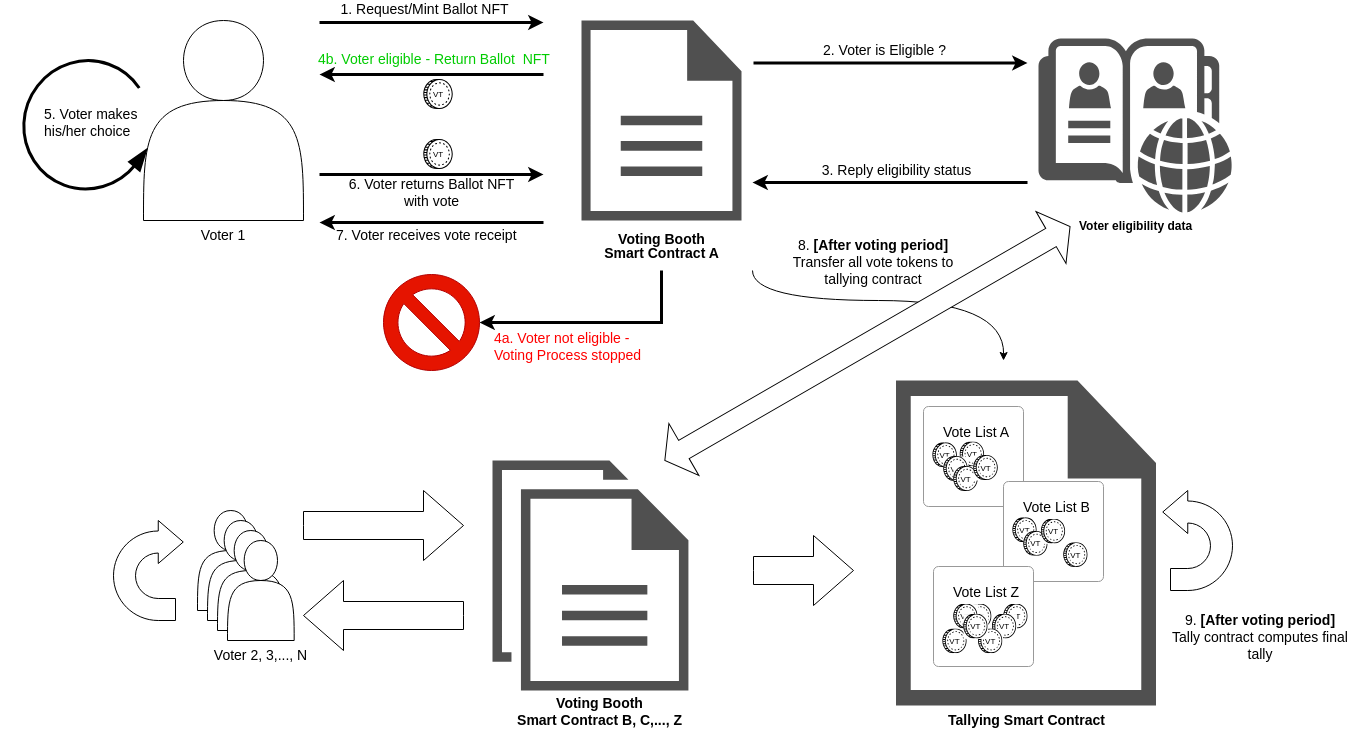
\includegraphics[width=0.7\textwidth]{../Images/03_account_based_solution.png}
    \caption{Account-based version of the e-voting system proposed.}
    \label{fig:account_based_architecture}
\end{figure}

The main difference with this approach is that, in this case, the Vote NFT is always stored under the account of the element that holds the token at a given point in the process, i.e., the Vote NFT is actually moved through distinct storage locations throughout the process, which are abstracted and referenced as accounts, as opposed to the contract-based approach, where the only changes are to the internal mappings of the NFT-generating contract, typically indicating which address controls which NFT. From a voter's perspective, he or she should not detect any changes in the voting experience.

\subsubsection{Account-based Blockchain to use}
For this case, we considered the Flow blockchain for two main reasons:

\begin{enumerate}
    \item{The creators of CryptoKitties \cite{Gharegozlou2019}, one of the first examples of an Ethereum NFT-generating smart contract, created the Flow blockchain in 2020 \cite{Hentschel2019}. Besides establishing one of the first real-world examples of digital collectibles, the CryptoKitties smart contract established a series of game-like characteristics designed to attract users to experiment with the concept.
          \par
          The success of this initiative exposed the potential behind NFT technology as well as how limited and difficult it really was to scale the Ethereum blockchain. The network experienced difficulties in responding to an unusually high volume of transactions due to the rapid popularity of CryptoKitties.
          \par
          Flow developed Cadence \cite{Cadence2023}, an interpretative programming language, to create smart contracts and expand the functionalities of this blockchain through automated Cadence-written scripts and transactions.}

    \item{Flow is an example of an account-based, resource-oriented blockchain. Given its claims of scalability, there was some emphasis on data storage when planning this blockchain, which is useful towards the system we intend to implement.}

\end{enumerate}

\subparagraph{Account model in Flow}
\label{flow_accounts}
An account in Flow consists of a record for a specific blockchain state. This record consists of:

\begin{itemize}
    \item{A unique, 8-byte long unique address.}
    \item{A pair of encryption keys used to interact with the account and verify the validity of digital signatures. \cite{flow2024}}.
    \item{A smart contract storage space to save contract code.}
    \item{The main storage space.}
\end{itemize}

Fig. \ref{fig:flow_account_model} illustrates this organisation.

\begin{figure}[htp]
    \centering
    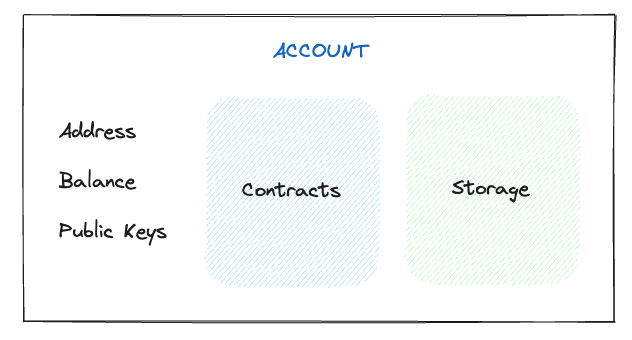
\includegraphics[width=0.7\textwidth]{../Images/Flow_account_model.png}
    \caption{Overview of the account model used in the Flow blockchain. Source: \cite{flow2024}}
    \label{fig:flow_account_model}
\end{figure}

An important fact to retain from Fig. \ref{fig:flow_account_model} is that contracts in this model are stored in a distinct area from general-purpose storage and, as such, have different access rules. Like with any other smart contract-capable blockchain, smart contracts in Flow can be read by anyone, even though they are stored in an account-specific storage area.

\paragraph{How storage works on Flow}
Flow stores data as digital objects. These objects can be defined as "resources," a special, highly regulated type of digital object in Flow. Resources are central to the functionality of this blockchain, so much so that its developers define the programming paradigm imposed by Cadence as a "resource-oriented paradigm" \cite{flow2024}.
\par
Storage in Flow is account-based. Address-based storage paths uniquely identify each digital object in storage. The internal mechanics of the Flow blockchain ensure that only the owner of an account can alter its storage, namely, read, write, and manipulate the access control (permissions) associated with data objects in storage.
\par
Cadence uses scripts and transactions to interact with Flow. Scripts are a sequence of instructions to execute in the blockchain but that do not change the state of the blockchain, i.e., scripts can only read data from the blockchain. Transactions are structurally similar to scripts, but these can change the state of the blockchain (move, create, and/or delete digital objects). As such, transactions require a digital signature by the owner of the account to modify.
\par
Similar to all other blockchains, storage space in Flow is not free, though it is arguably cheaper than in other popular blockchains such as Ethereum. The amount of storage allocated to an account is proportional to the balance of the FLOW token (Flow's native cryptocurrency, from here referred to in all capitals to distinguish it from the main blockchain) of the account in question, establishing a rate of 100MB of storage space per FLOW token, i.e., a user with a balance of 1 FLOW in his/her account can store up to 100MB of data in storage \cite{flow2024}. If an operation (transaction or smart contract function) stores data above the allowed capacity of an account based on the current balance, the transaction fails and all state changes are reverted, just like with a regular smart contract exception.
\par
Flow also establishes a base value of 100 kB of storage space that remains available in perpetuity. This establishes two consequences:

\begin{enumerate}
    \item {A user needs to pay to create an account. The "permanent" storage costs 0.001 FLOW, according to the rate mentioned above, and has to be paid during account creation, though these tokens actually end up in the main account balance.}
    \item {Flow accounts require a minimum balance of 0.001 FLOW at all times to pay for this permanent storage; therefore, Flow accounts cannot be completely emptied \cite{flow2024}.}
\end{enumerate}

\subparagraph{Storage domains}
\label{storage_domains}
Each account in Flow has two domains that define its storage space: \textit{/storage} and \textit{/public} \cite{flow2024}. Flow uses UNIX-style paths to reinforce the notion that these are used to uniquely identify a digital object in a storage area, similar to the path of a file or directory in a UNIX system.
\par
All resources stored in an account's storage go into the \textit{/storage} domain by default. Only the account owner(s) have access to this domain, for both write and read privileges. This means that any resource transferred into an account, either through a transaction or a functionally equivalent smart contract function, becomes private by default as soon as it is stored. To allow for external access, the controlling user must move that resource to either the \textit{/public} or \textit{/private} domains. Data in the \textit{/public} domain is available to everyone. The \textit{/private} domain, despite the name, actually sits somewhere between the \textit{/storage} and \textit{/public} domains regarding access. Data stored in this domain is only available to the owner and to users previously authorised by the owner.

\subparagraph{Capabilities}
\label{capabilities_references}
\textit{Capabilities} are tools used in the Flow blockchain to delegate access to resources (data objects). An account controller creates \textit{capabilities}, which are akin to a memory pointer in that instead of referencing a memory position, they reference a specific resource stored in the account where the \textit{capability} was created. \textit{Capability} creation changes the state of the blockchain; therefore, it needs to be done in a transaction digitally signed by the account owner to be executed. These requisites restrict the creation of \textit{capabilities} to the owner of the resource in question.
\par
Flow distributes \textit{capabilities} among account holders using a messaging system. Once created, the account owner publishes the \textit{capability} to the \textit{/public} domain of his/her account storage. From here, other users can \textit{borrow} (Flow names the API function used to retrieve a reference as \textit{borrow} to reinforce this notion) a reference to the object from the capability.

\end{document}